\documentclass[10pt,a4paper]{article}

\usepackage[utf8]{inputenc}
\usepackage[T1]{fontenc}
\usepackage{lmodern}
\usepackage{graphicx}
\usepackage{color}
\usepackage{xcolor}
\usepackage{geometry}
\usepackage{parskip}
\usepackage[brazil]{babel}
\usepackage[hidelinks]{hyperref}
\usepackage{listings}
\usepackage{placeins}

\geometry{
  a4paper,
  left=2cm,
  right=2cm,
  top=2cm,
  bottom=2cm,
}

\definecolor{dkgreen}{rgb}{0,0.4,0}
\definecolor{dkblue}{rgb}{0,0,0.6}
\definecolor{dkred}{rgb}{0.5,0,0}
\definecolor{ltblue}{rgb}{0.1,0.1,0.9}
\definecolor{gray}{rgb}{0.5,0.5,0.5}
\definecolor{green}{rgb}{0,0.6,0}
\definecolor{orange}{rgb}{0.75,0.25,0}
\colorlet{lessOrange}{orange!70!gray}

\lstset{frame=tb,
	language=C++,
	aboveskip=3mm,
	belowskip=3mm,
	showstringspaces=false,
	columns=flexible,
	basicstyle={\small\ttfamily},
	numbers=none,
	literate={~}{{\raisebox{-0.7ex}{\texttt{\char`~}}}}1,
	numberstyle=\tiny\color{gray},
	keywordstyle=\color{dkblue},
	commentstyle=\color{gray},
	identifierstyle=\color{lessOrange},
	morecomment=[l][\color{dkgreen}]{\#},
	stringstyle=\color{dkgreen},
	breaklines=true,
	breakatwhitespace=true,
	tabsize=4,
	morekeywords={
		uniform, layout, in, out, vec2, vec3, vec4, mat2, mat3, mat4,
		sampler2D, samplerCube, discard, image2D, readonly, ivec2,
		GLuint, GLint, GLchar, GLsizei, GLenum, GLfloat, GLboolean,
		GLvoid, GLbitfield, GLsync, GLuint64, GLintptr, GLsizeiptr,
		atomic_uint, flat, smooth
	}
}

\title{\vspace{-2cm}\bfseries Trabalho Prático 1 - Equações Diferenciais Numéricas}
\author{Artur Fonseca Costa}
\date{}

\begin{document}

\maketitle



\section{Introdução}

O repositório, \href{https://github.com/Tuzass/EDN}{disponível aqui}, contém o código completo, assim como as instruções de compilação. Aqui, serão mostrados apenas os trechos de código relevantes para a demonstração dos resultados.



\section{Métodos de Runge-Kutta}\label{sec:introducao}

\subsection{Ordem 2}

Tem-se o PVI $y' = -y + 2 \cos x; y(0) = 1$, cuja solução exata é $\varphi(x) = \sin x + \cos x$. Foi implementado o método de Runge-Kutta de 2 estágios:

\begin{lstlisting}
	// Runge-Kutta method with 2 stages
	void rk2Method(double x_0, double X, double y_0, double h, double b_2){
		const int N = (X - x_0) / h;
		std::vector<double> x(N + 1);
		std::vector<double> y(N + 1);
		x[0] = x_0;
		y[0] = y_0;

		for (int j = 1; j <= N; j++){
			double k_1 {f(x[j - 1], y[j - 1])};
			double k_2 {f(x[j - 1] + (0.5 * h / b_2), y[j - 1] + 0.5 * h * k_1 / b_2)};

			x[j] = x[0] + j * h;
			y[j] = y[j - 1] + h * (1 - b_2) * k_1 + h * b_2 * k_2;
		}
	}
\end{lstlisting}
Se $\texttt{b\_2} = \frac{1}{2}$, tem-se o método de Heun; se $\texttt{b\_2} = 1$, tem-se o método do ponto médio. Ambos os métodos foram testados com $h = 1$, $h = 0.1$, e $h = 0.01$. Os resultados, assim como a ordem dos erros, são mostradas abaixo:

\begin{figure}[ht!]
	\centering
	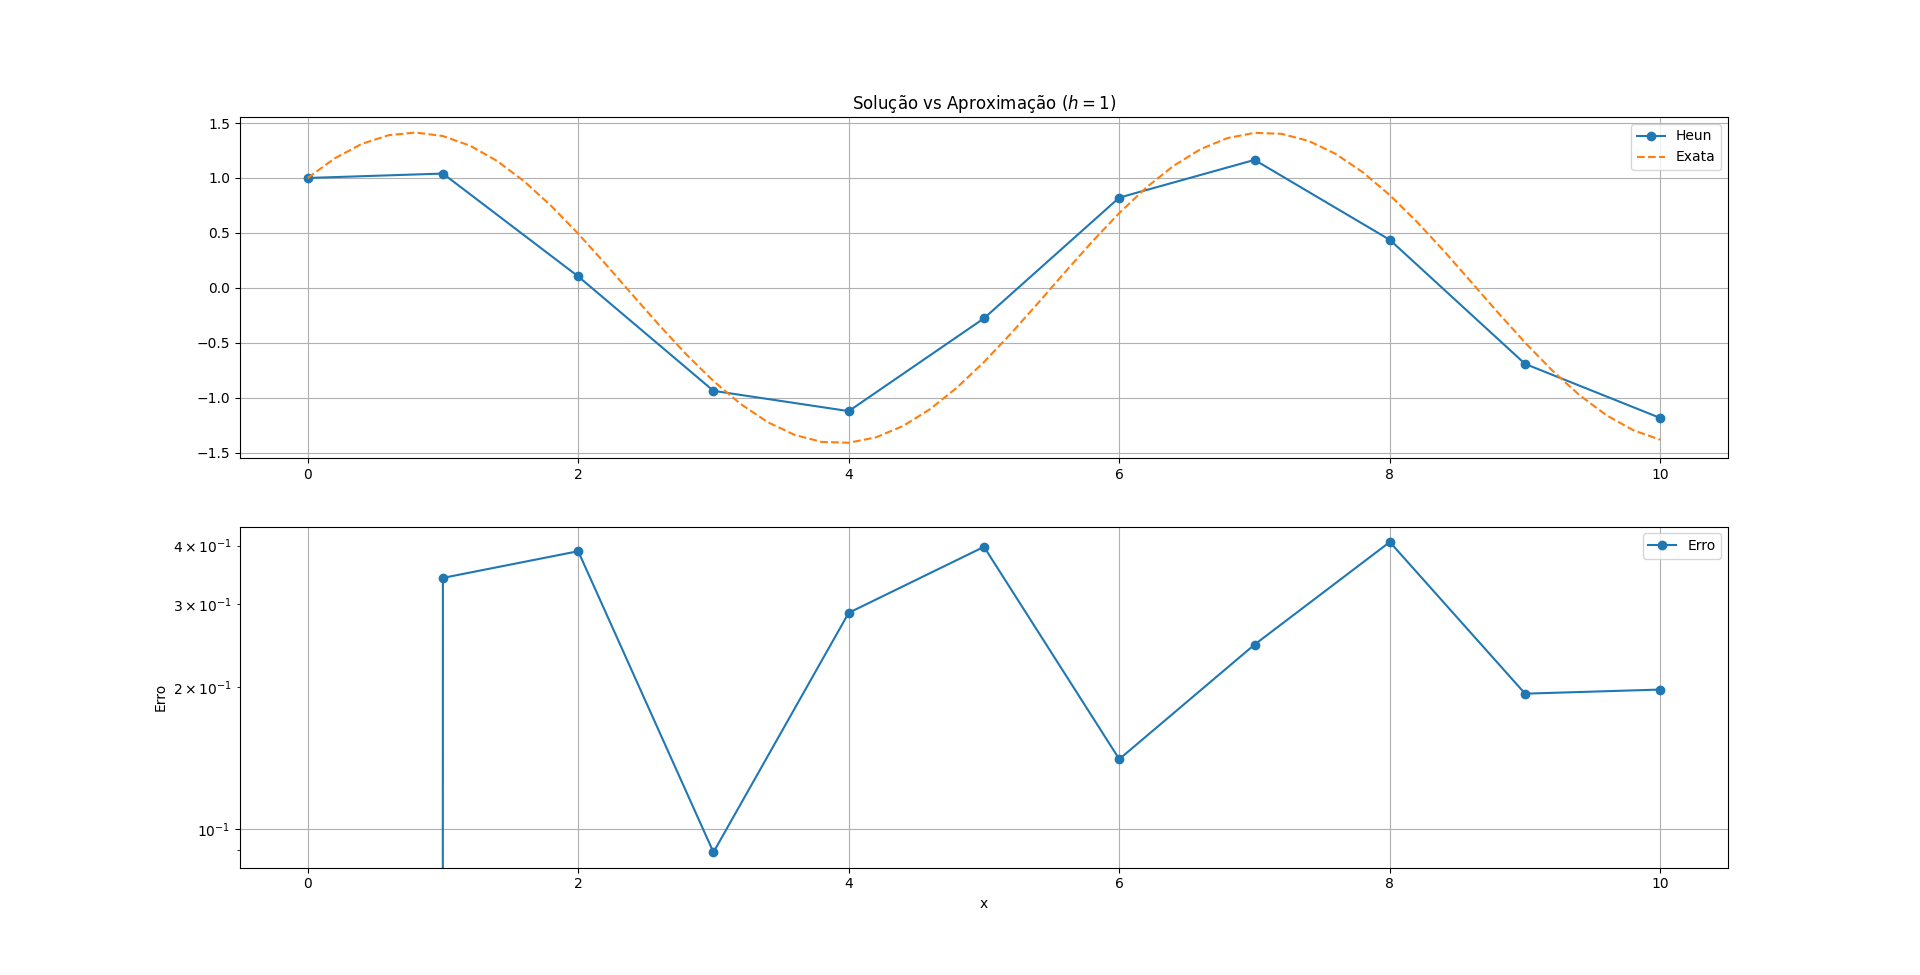
\includegraphics[width=0.8\textwidth]{img/2/heun_1.png}
\end{figure}

\begin{figure}
	\centering
	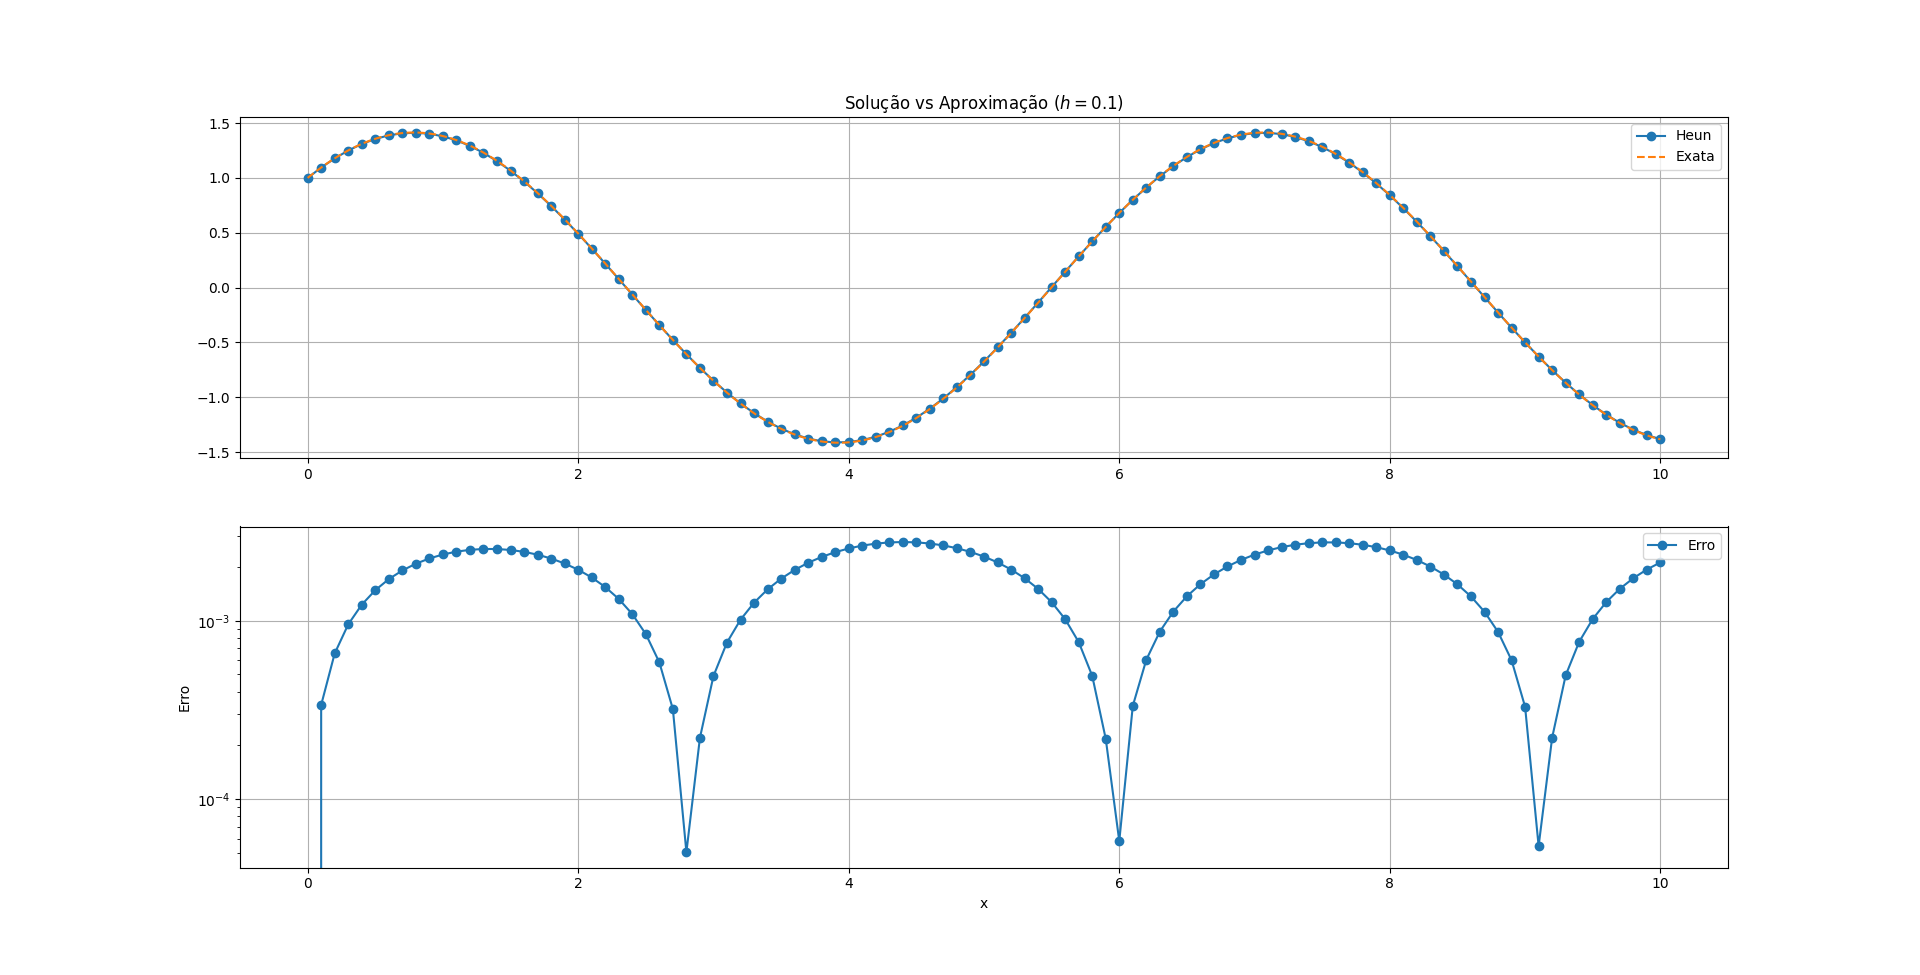
\includegraphics[width=0.7\textwidth]{img/2/heun_01.png}
	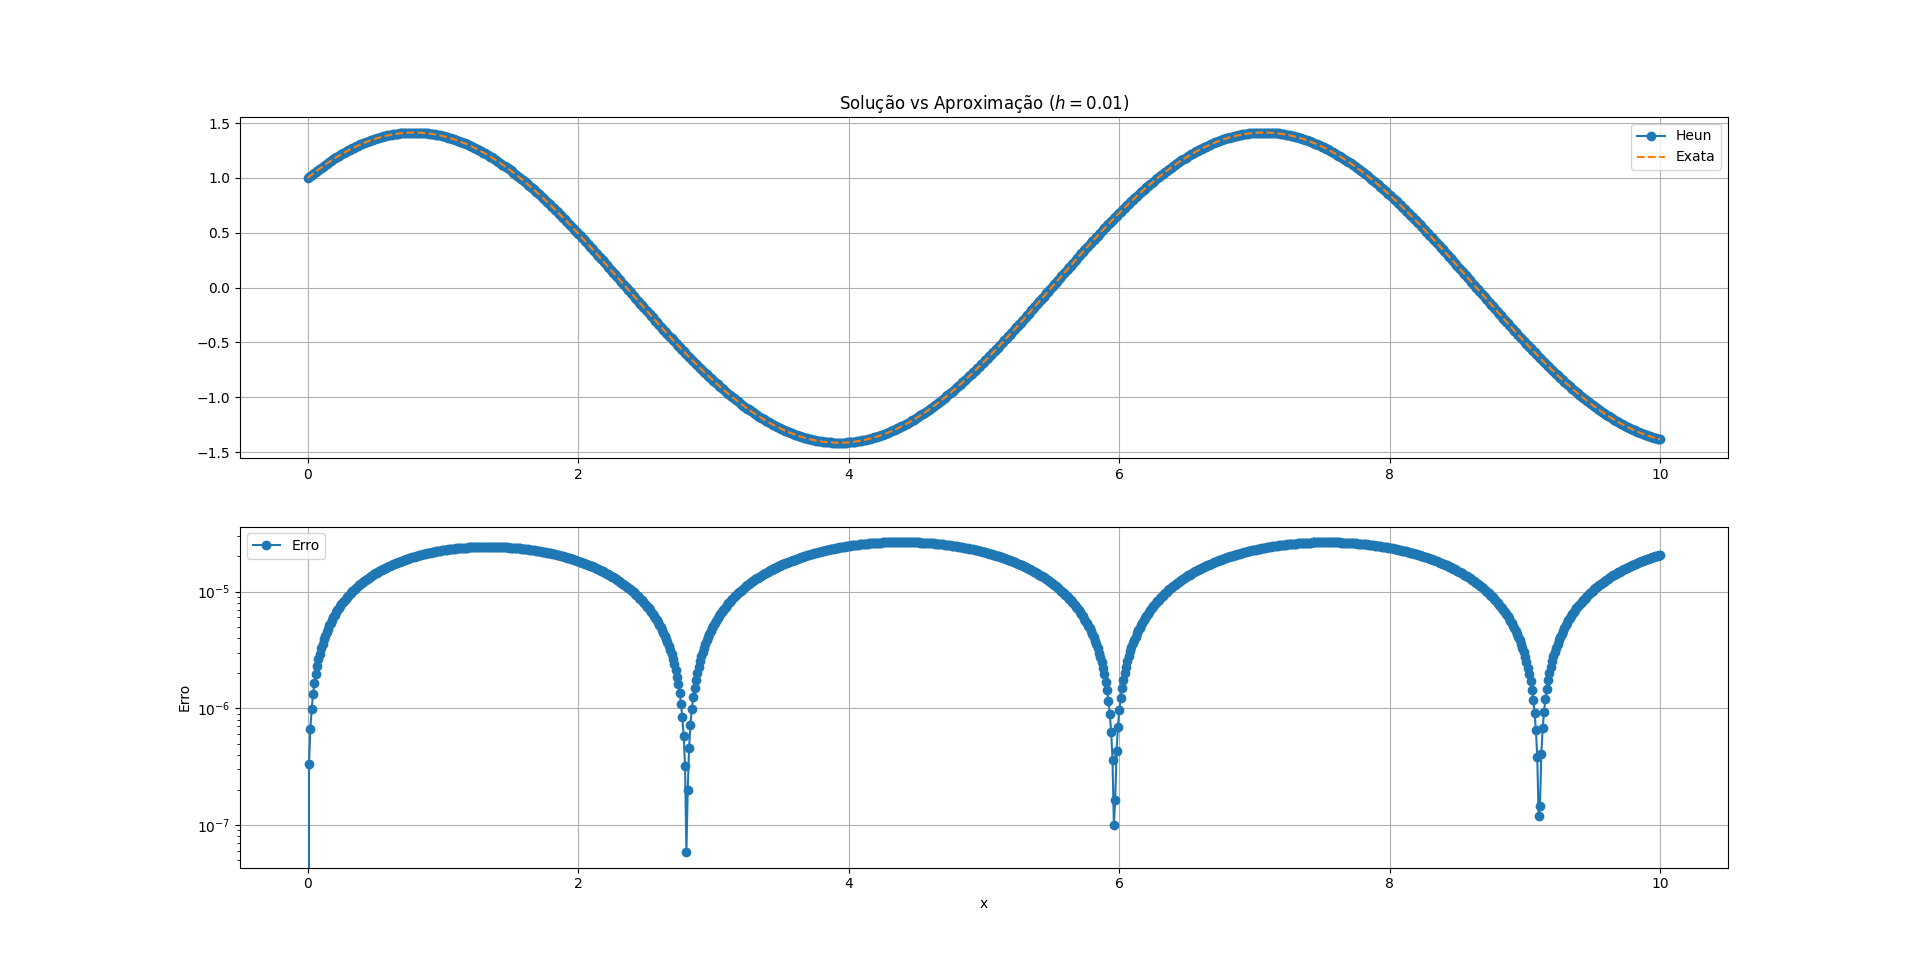
\includegraphics[width=0.7\textwidth]{img/2/heun_001.png}
	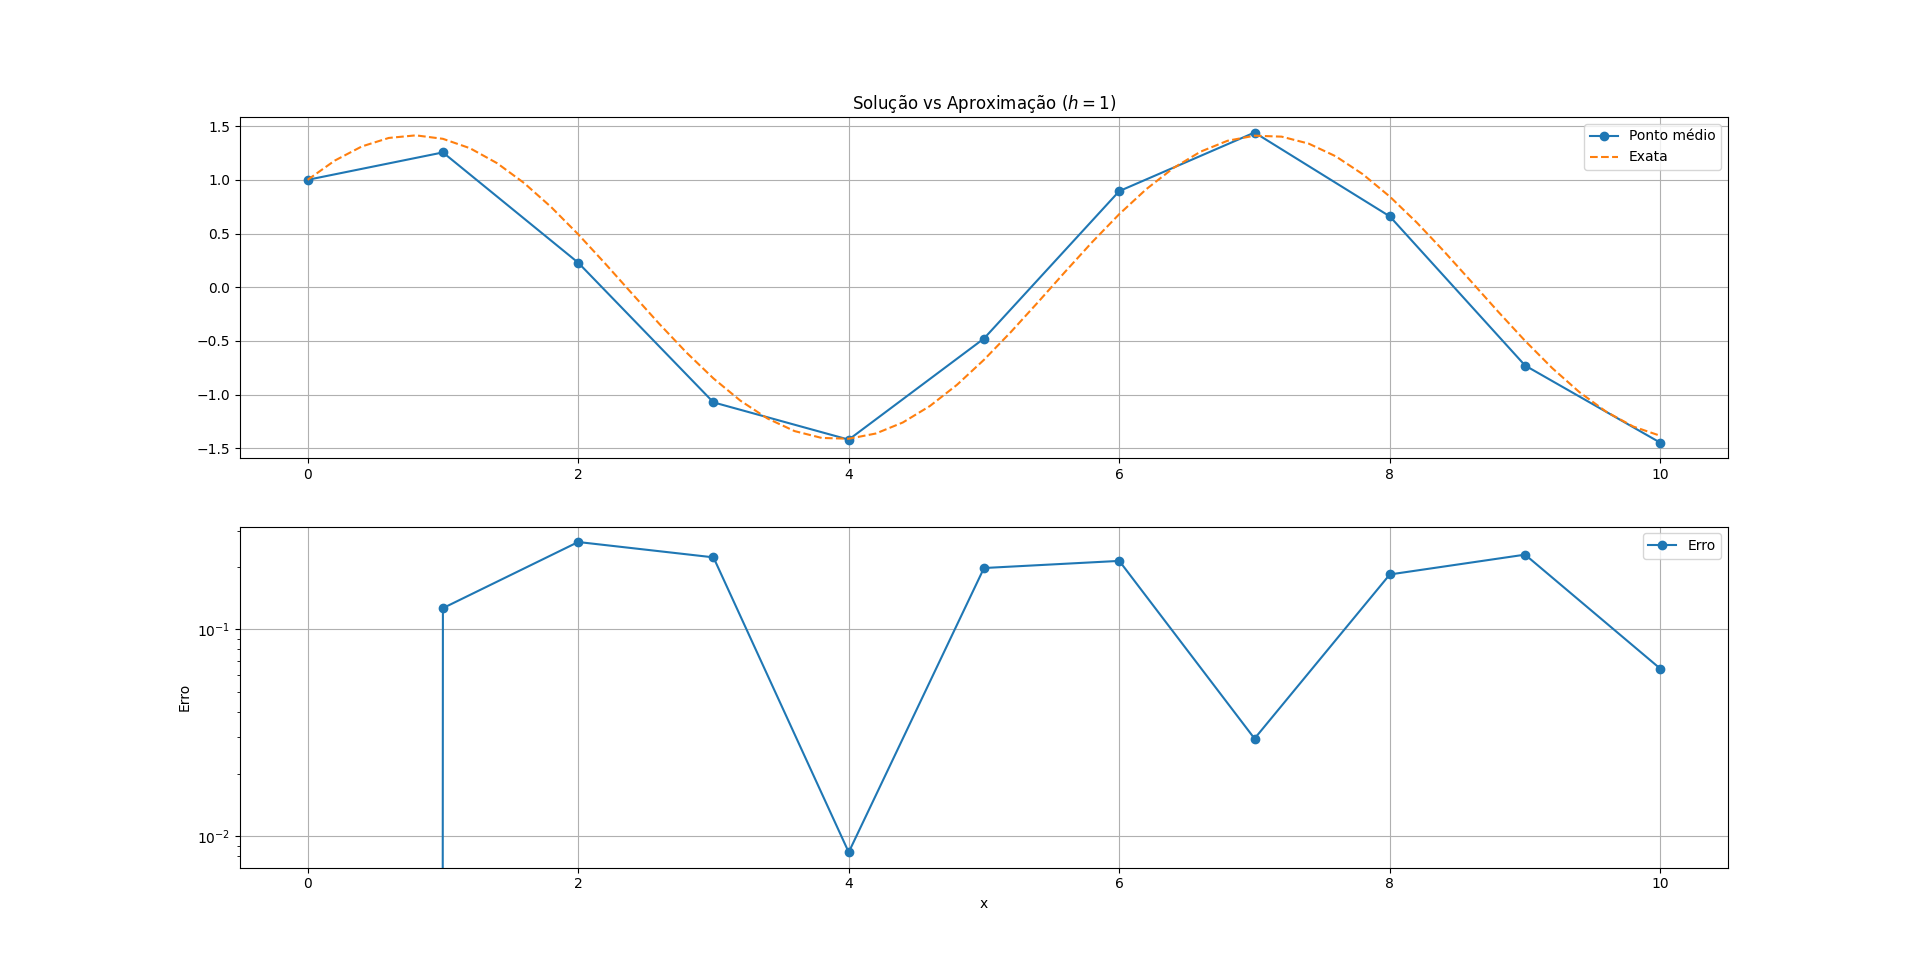
\includegraphics[width=0.7\textwidth]{img/2/midpoint_1.png}
	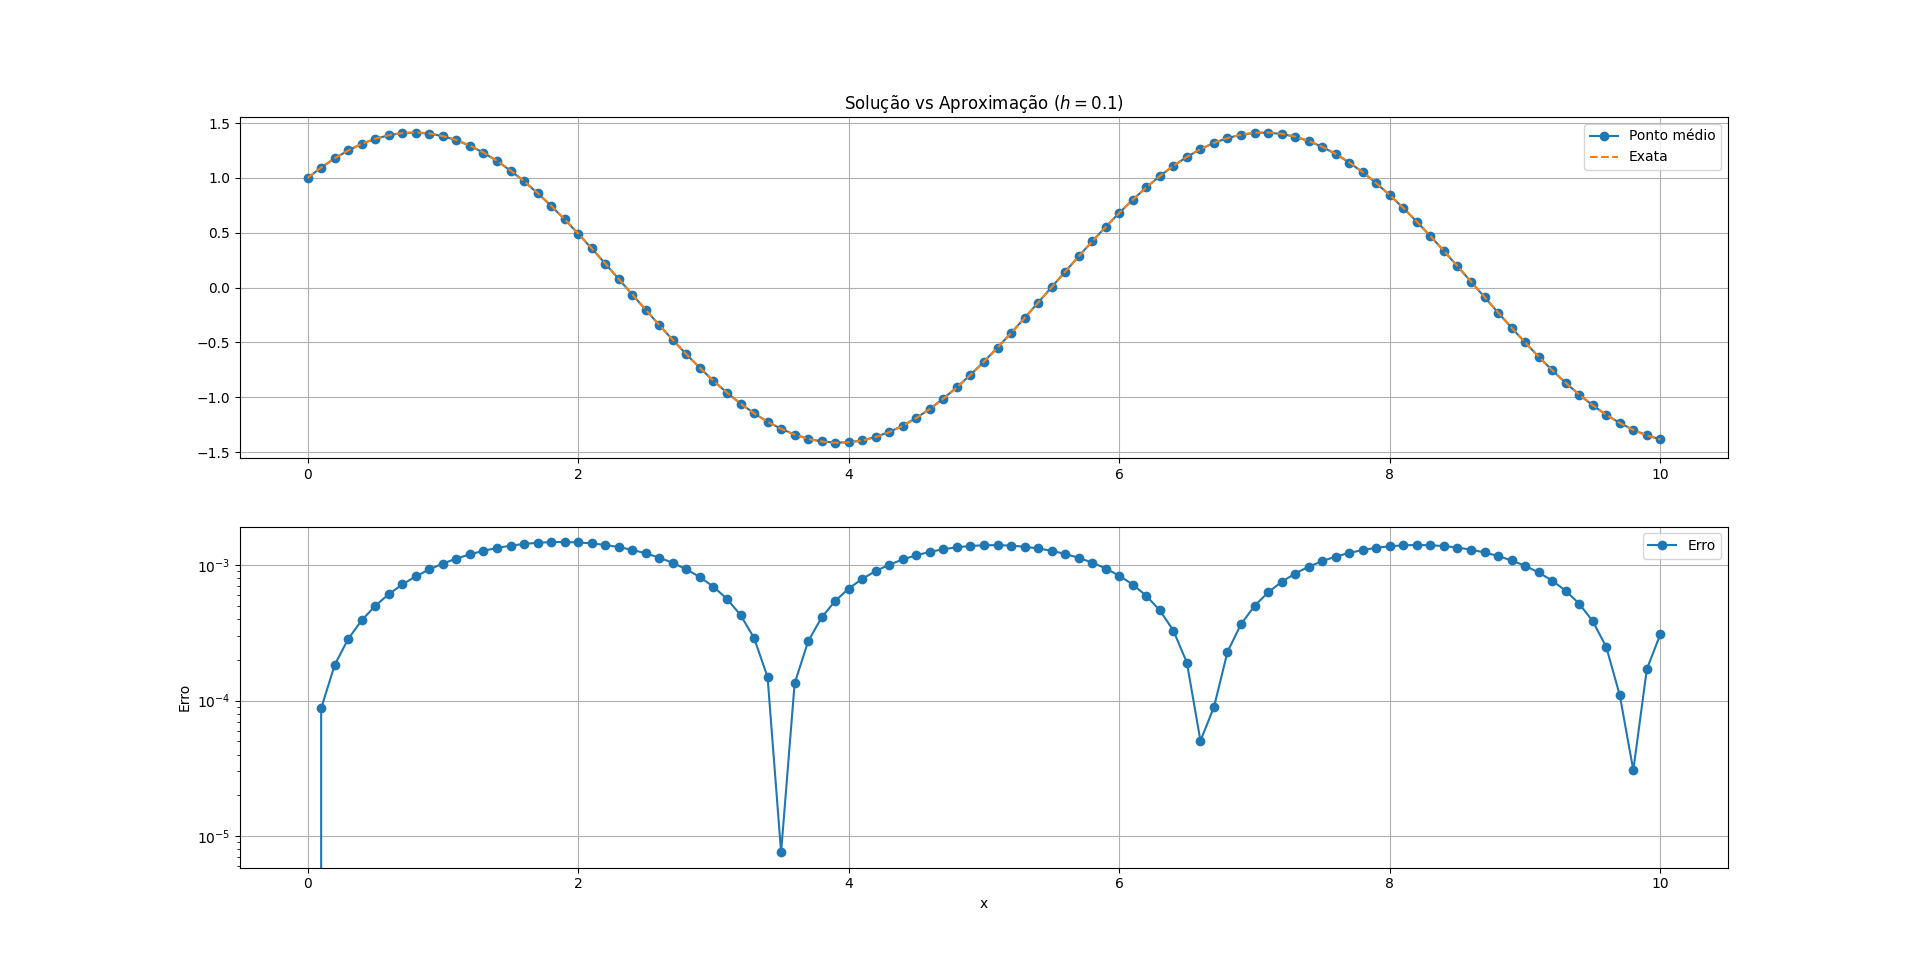
\includegraphics[width=0.7\textwidth]{img/2/midpoint_01.png}
\end{figure}

\begin{figure}[ht!]
	\centering
	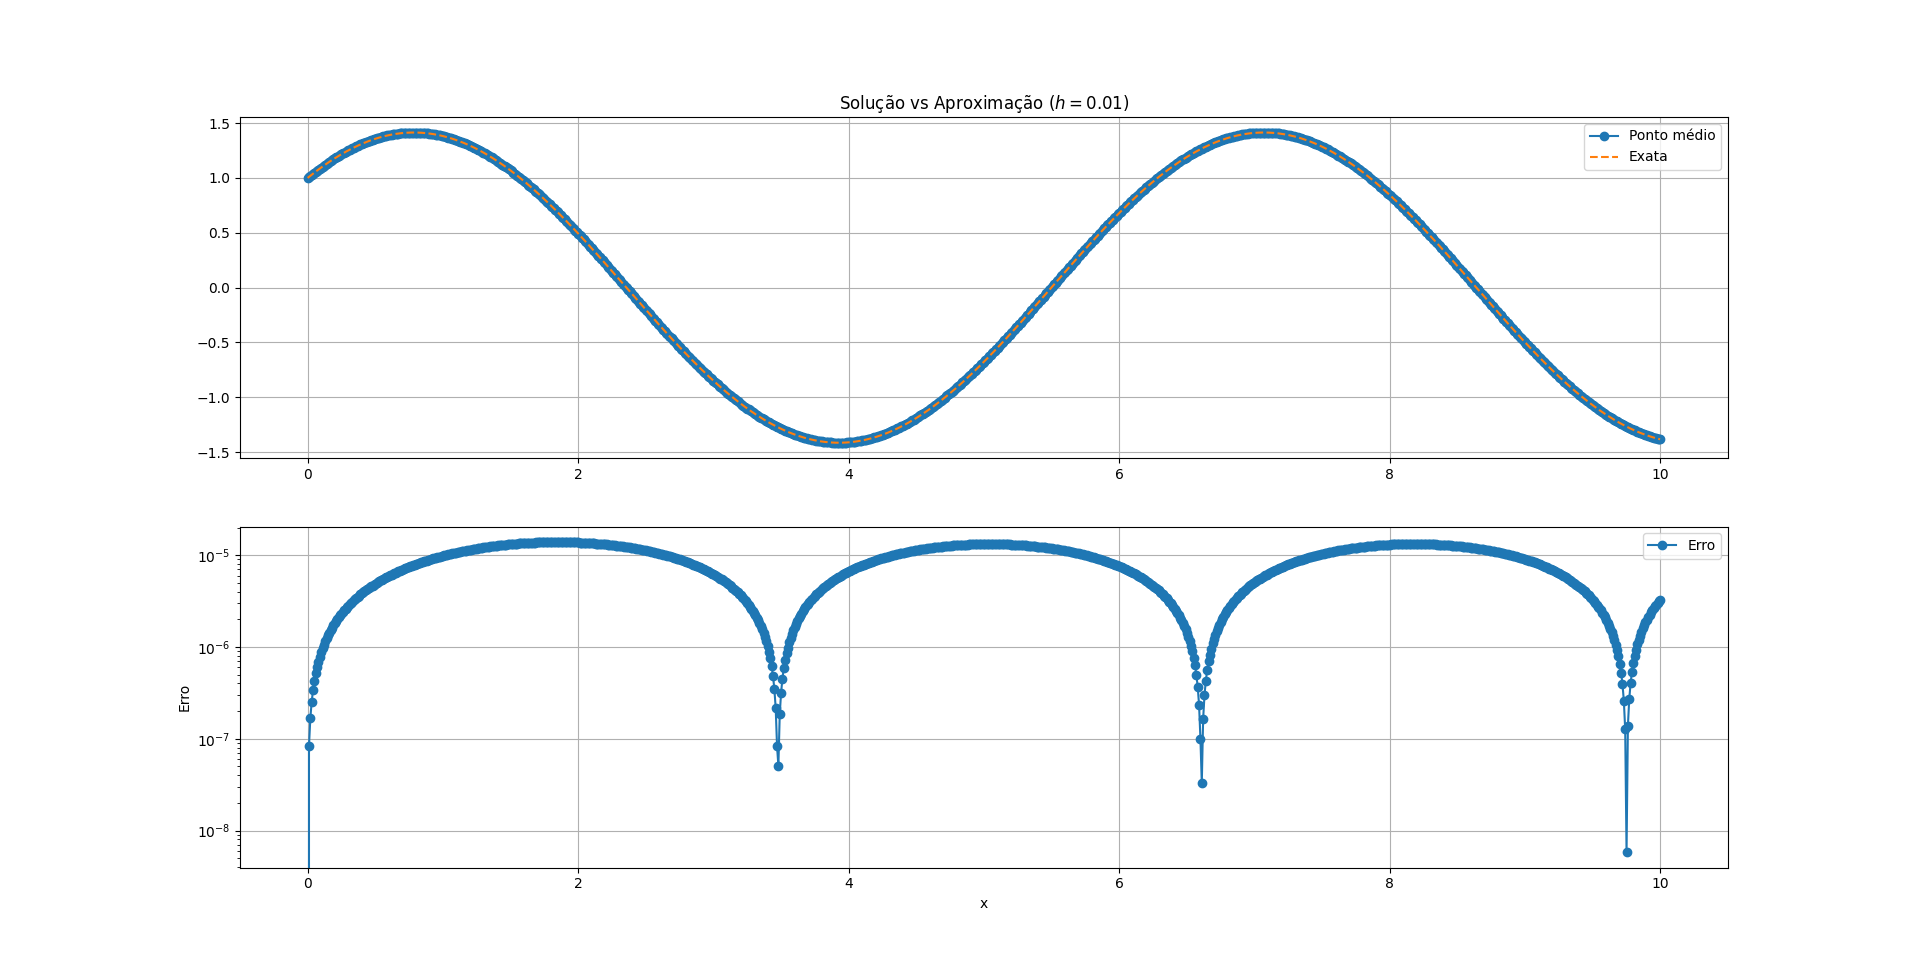
\includegraphics[width=0.7\textwidth]{img/2/midpoint_001.png}
\end{figure}

\FloatBarrier

Como esperado, o erro desses métodos é $O(h^2)$. Mesmo com o valor altíssimo $h = 1$, o erro mantém esse comportamento e o resultado é uma aproximação razoável dado o número minúsculo de iterações.

\subsection{Ordem Superior}

Foi implementado o método de Runge-Kutta de 4 estágios, cujo erro é $O(h^4)$:

\begin{lstlisting}
	// Runge-Kutta method with 4 stages
	void rk4Method(double x_0, double X, double y_0, double h){
		const int N = (X - x_0) / h;
		std::vector<double> x(N + 1);
		std::vector<double> y(N + 1);
		x[0] = x_0;
		y[0] = y_0;

		for (int j = 1; j <= N; j++){
			double k_1 {f(x[j - 1], y[j - 1])};
			double k_2 {f(x[j - 1] + 0.5 * h, y[j - 1] + 0.5 * h * k_1)};
			double k_3 {f(x[j - 1] + 0.5 * h, y[j - 1] + 0.5 * h * k_2)};
			double k_4 {f(x[j - 1] + h, y[j - 1] + h * k_3)};

			x[j] = x[0] + j * h;
			y[j] = y[j - 1] + h * (k_1 + 2 * k_2 + 2 * k_3 + k_4) / 6;
		}
	}
\end{lstlisting}
Os resultados, assim como a ordem dos erros, são mostradas abaixo:

\begin{figure}[ht!]
	\centering
	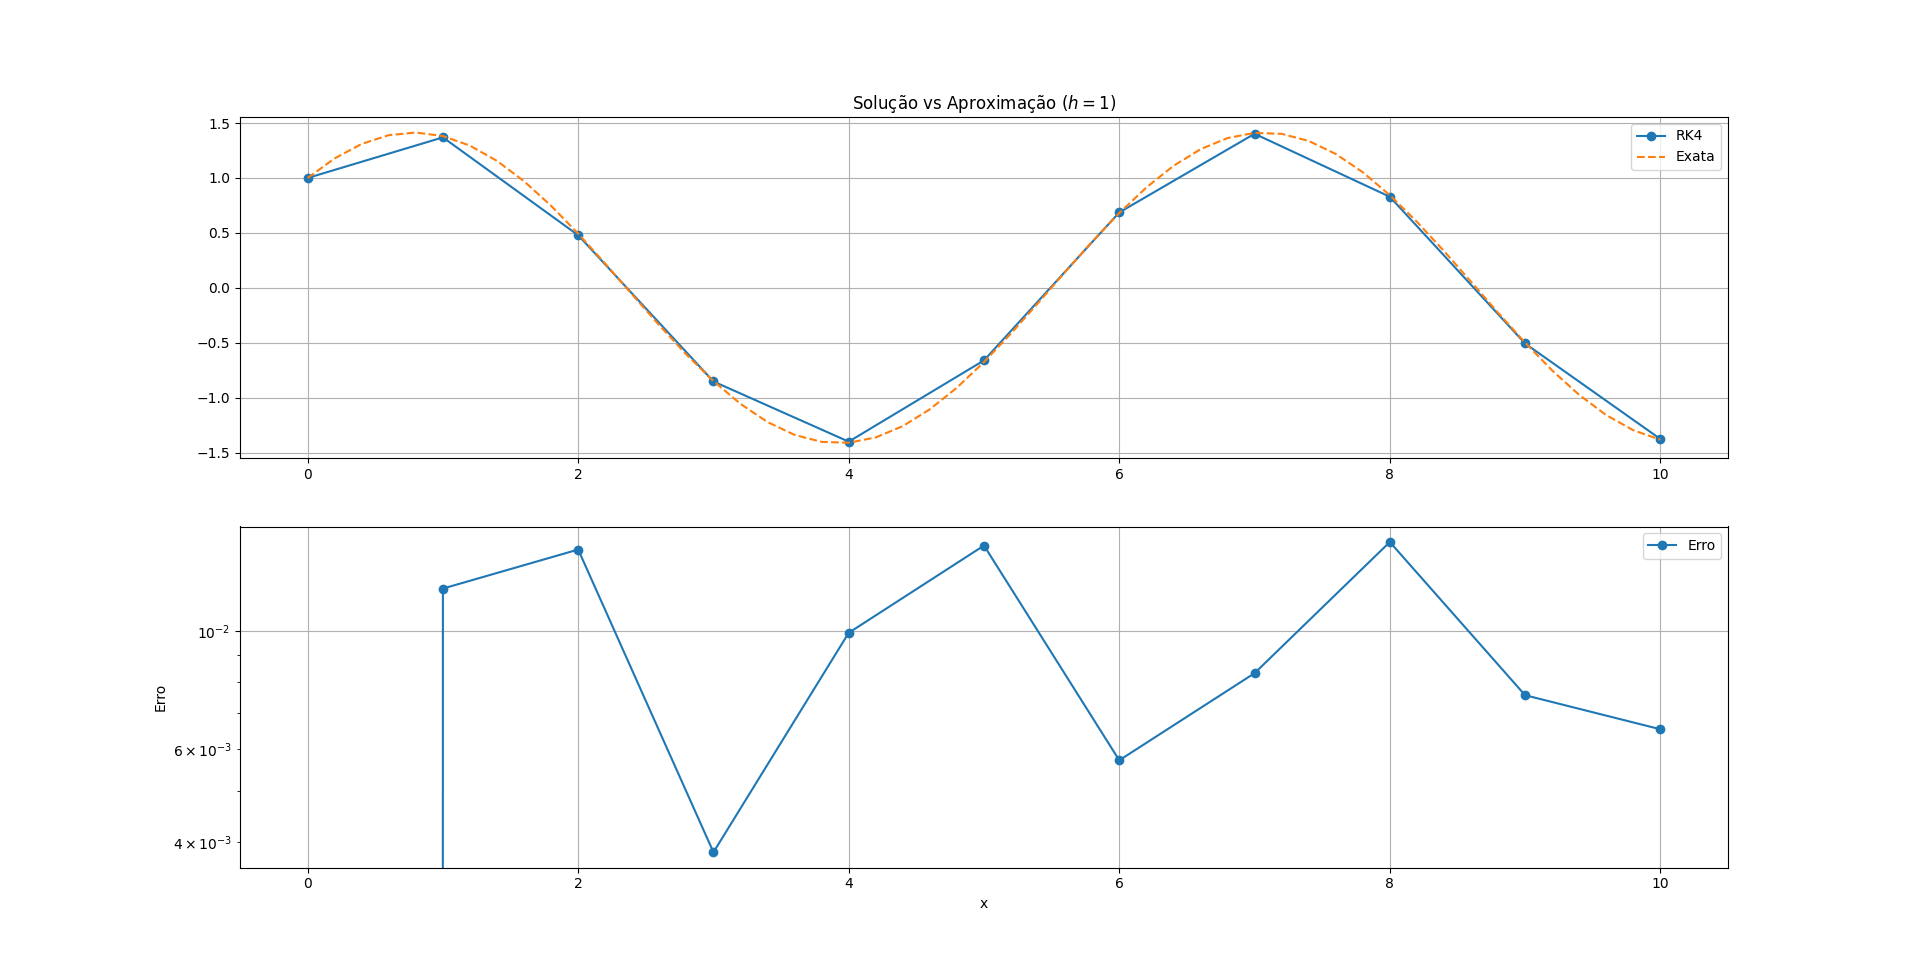
\includegraphics[width=0.7\textwidth]{img/2/rk4_1.png}
\end{figure}

\begin{figure}[ht!]
	\centering
	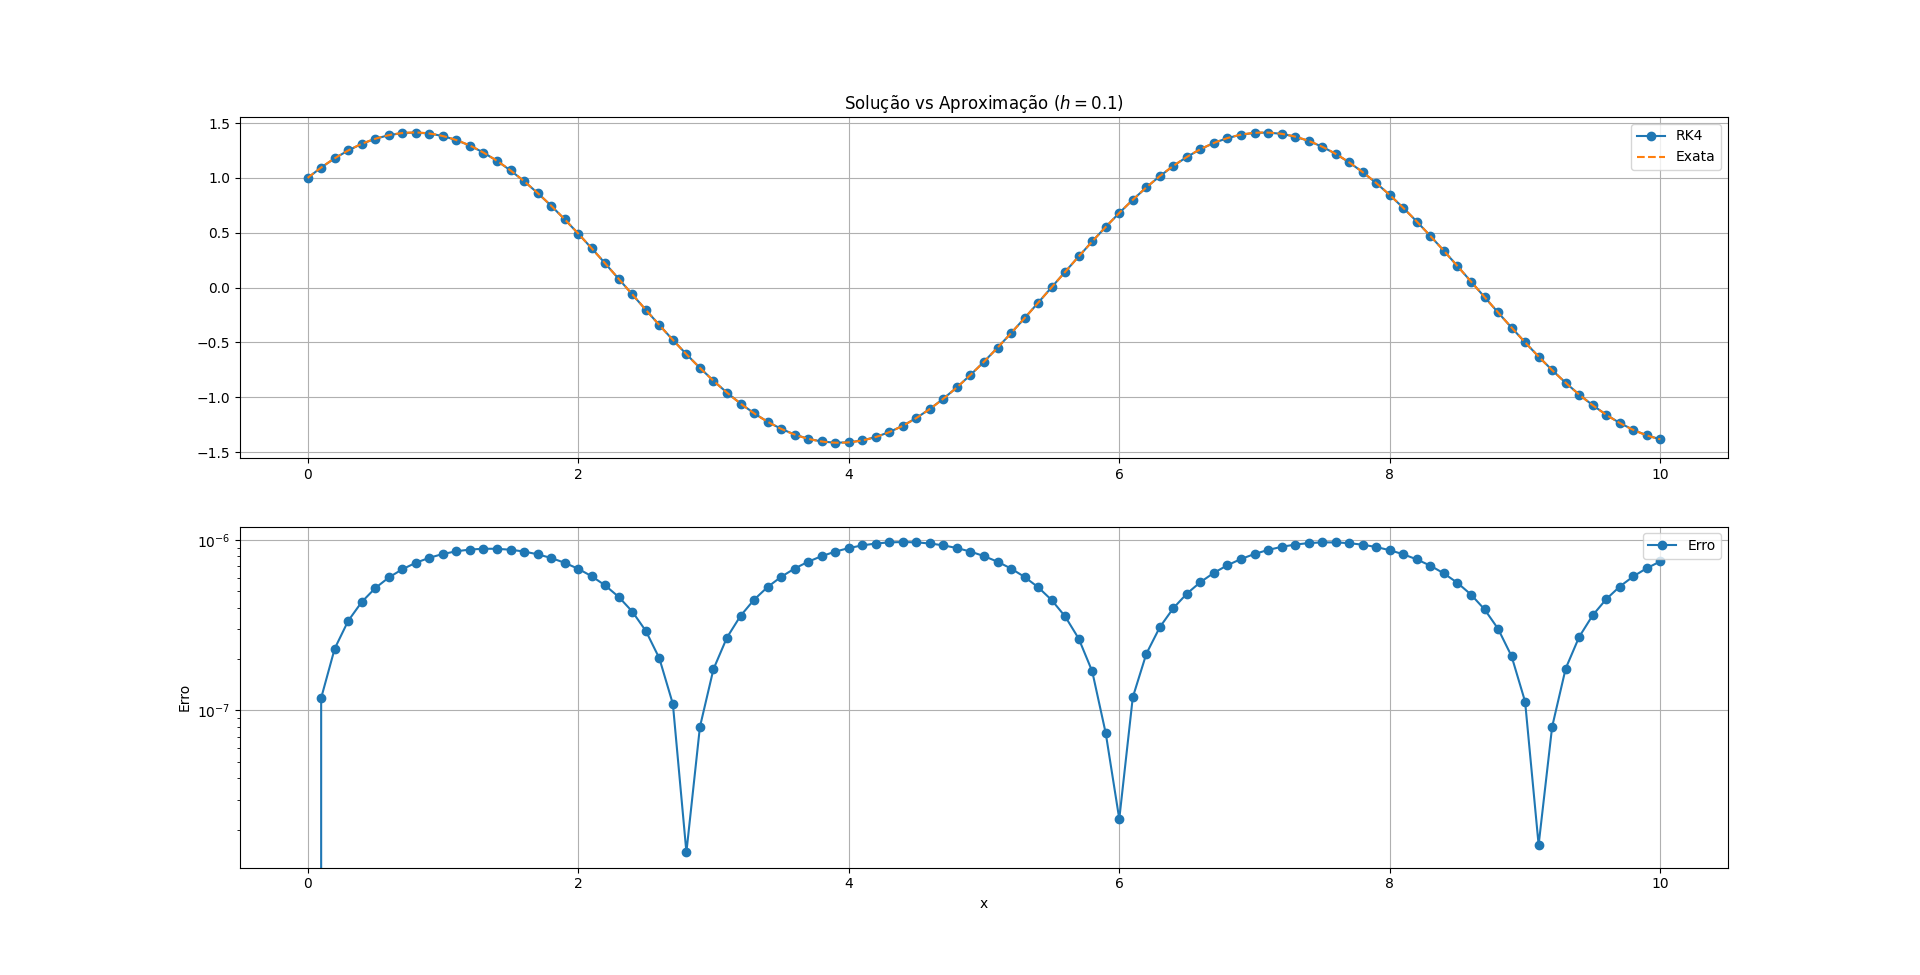
\includegraphics[width=0.7\textwidth]{img/2/rk4_01.png}
	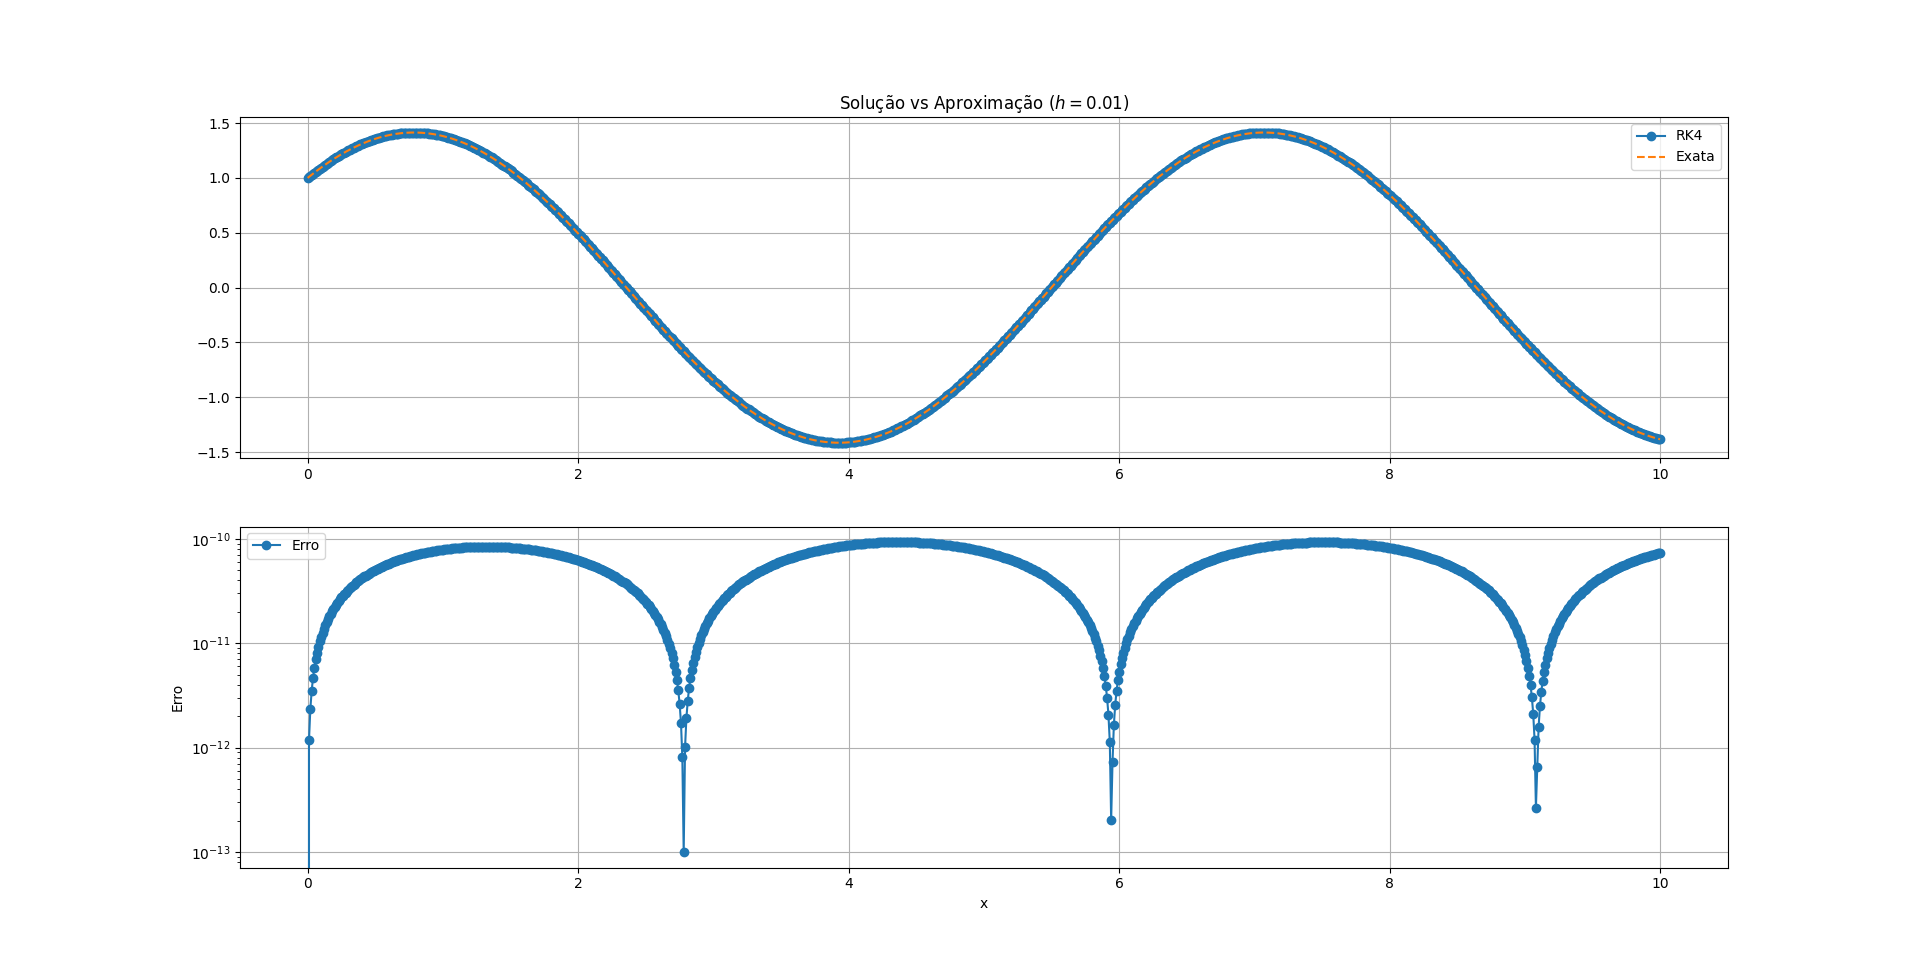
\includegraphics[width=0.7\textwidth]{img/2/rk4_001.png}
\end{figure}

\FloatBarrier

Mais uma vez, o erro se comporta como esperado. No entanto, é necessário pontuar que o número de operações do método RK4 é apenas duas vezes maior que do método RK2, ao mesmo tempo em que o erro é $O(h^4)$. Por se tratar de uma função muito simples, os erros estavam cerca de 2 ordens de magnitude abaixo do esperado. Não foi testado o valor $h = 0.001$, pois os erros seriam da ordem de $10^{-14}$, estando muito próximos do limite de precisão da máquina.



\section{Métodos Implícitos de Passo Único}\label{sec:introducao}

\subsection{Implementação de Problemas Lineares}

Tem-se o PVI $y' = x e^{-x}; y(0) = 0$ (há um pequeno erro no enunciado em que $y(0) = 1$, porém este não é o valor da solução exata no ponto $x = 0$), cuja solução exata é $\varphi(x) = \frac{x^2}{2} e^{-x}$. Tratando-se de métodos implícitos de passo único, foi implementado o método Theta:

\begin{lstlisting}
	// implicit theta method; num_corrections indicates how many corrections in the predictor-corrector scheme
	void thetaMethod(double x_0, double X, double y_0, double h, double theta, int num_corrections){
		const int N = (X - x_0) / h;
		std::vector<double> x(N + 1);
		std::vector<double> y(N + 1);
		x[0] = x_0;
		y[0] = y_0;

		for (int j = 1; j <= N; j++){
			double y_approx = y[j - 1] + h * f(x[j - 1], y[j - 1]); // first approximation given by Euler's method
			x[j] = x[0] + j * h;

			for (int k = 1; k <= num_corrections; k++){
				y_approx = y[j - 1] + h * ((1 - theta) * f(x[j - 1], y[j - 1]) + theta * f(x[j], y_approx));
			}

			y[j] = y_approx;
		}
	}
\end{lstlisting}
Se $\theta = 1$, tem-se o método de Euler regressivo; se $\theta = \frac{1}{2}$, tem-se o método Trapezoidal.

Em métodos implícitos, existe a necessidade de resolver uma equação implícita para obter o valor de $y_{j + 1}$. Algumas opções incluem aproximações sucessivas, até que duas aproximações consecutivas sejam arbitrariamente próximas, o método de Newton para encontrar raízes, ou um esquema preditor-corretor.

Foi implementada a última opção, usando o método de Euler como esquema preditor para obter $y_0$. O esquema corretor é aplicado um número fixo de vezes. Foram testadas 2 e 5 correções por $y_j$, porém sem nenhuma mudança significativa. Serão mostrados os resultados obtidos com 2 correções. Mais uma vez, o erro manteve-se dentro da ordem esperada.

\begin{figure}[ht!]
	\centering
	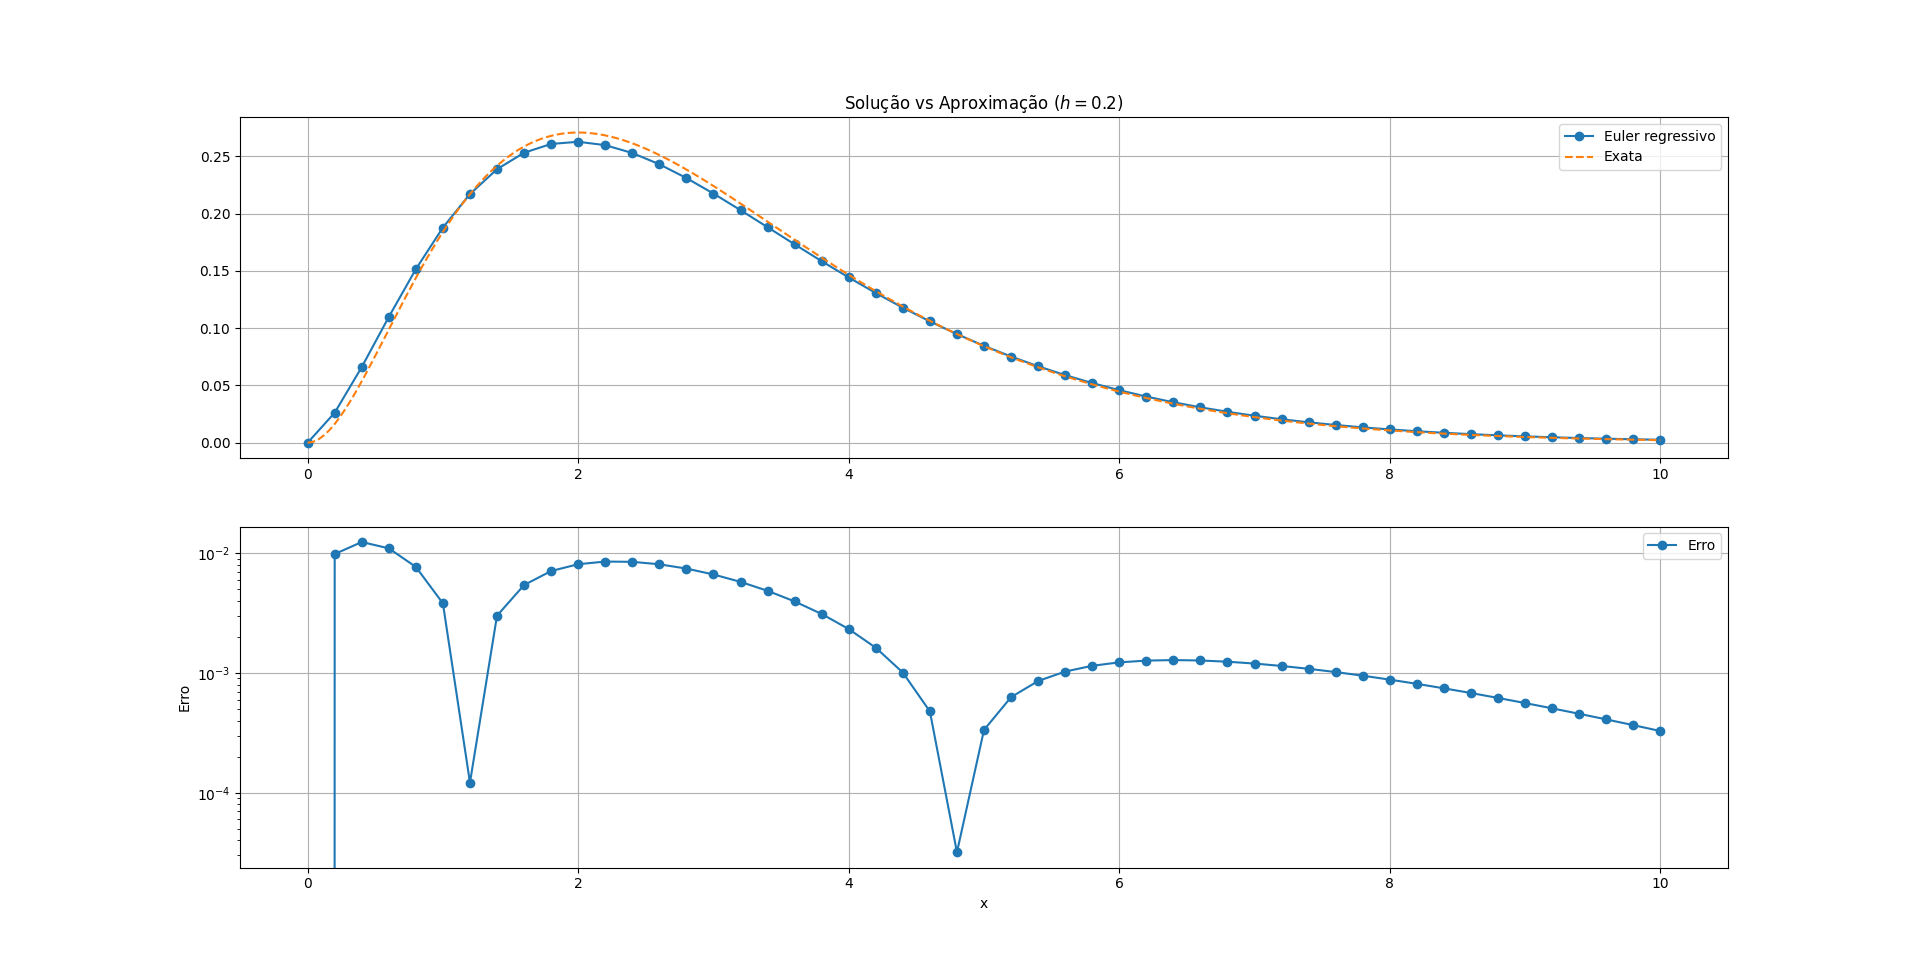
\includegraphics[width=0.7\textwidth]{img/3/implicit_02_2.png}
	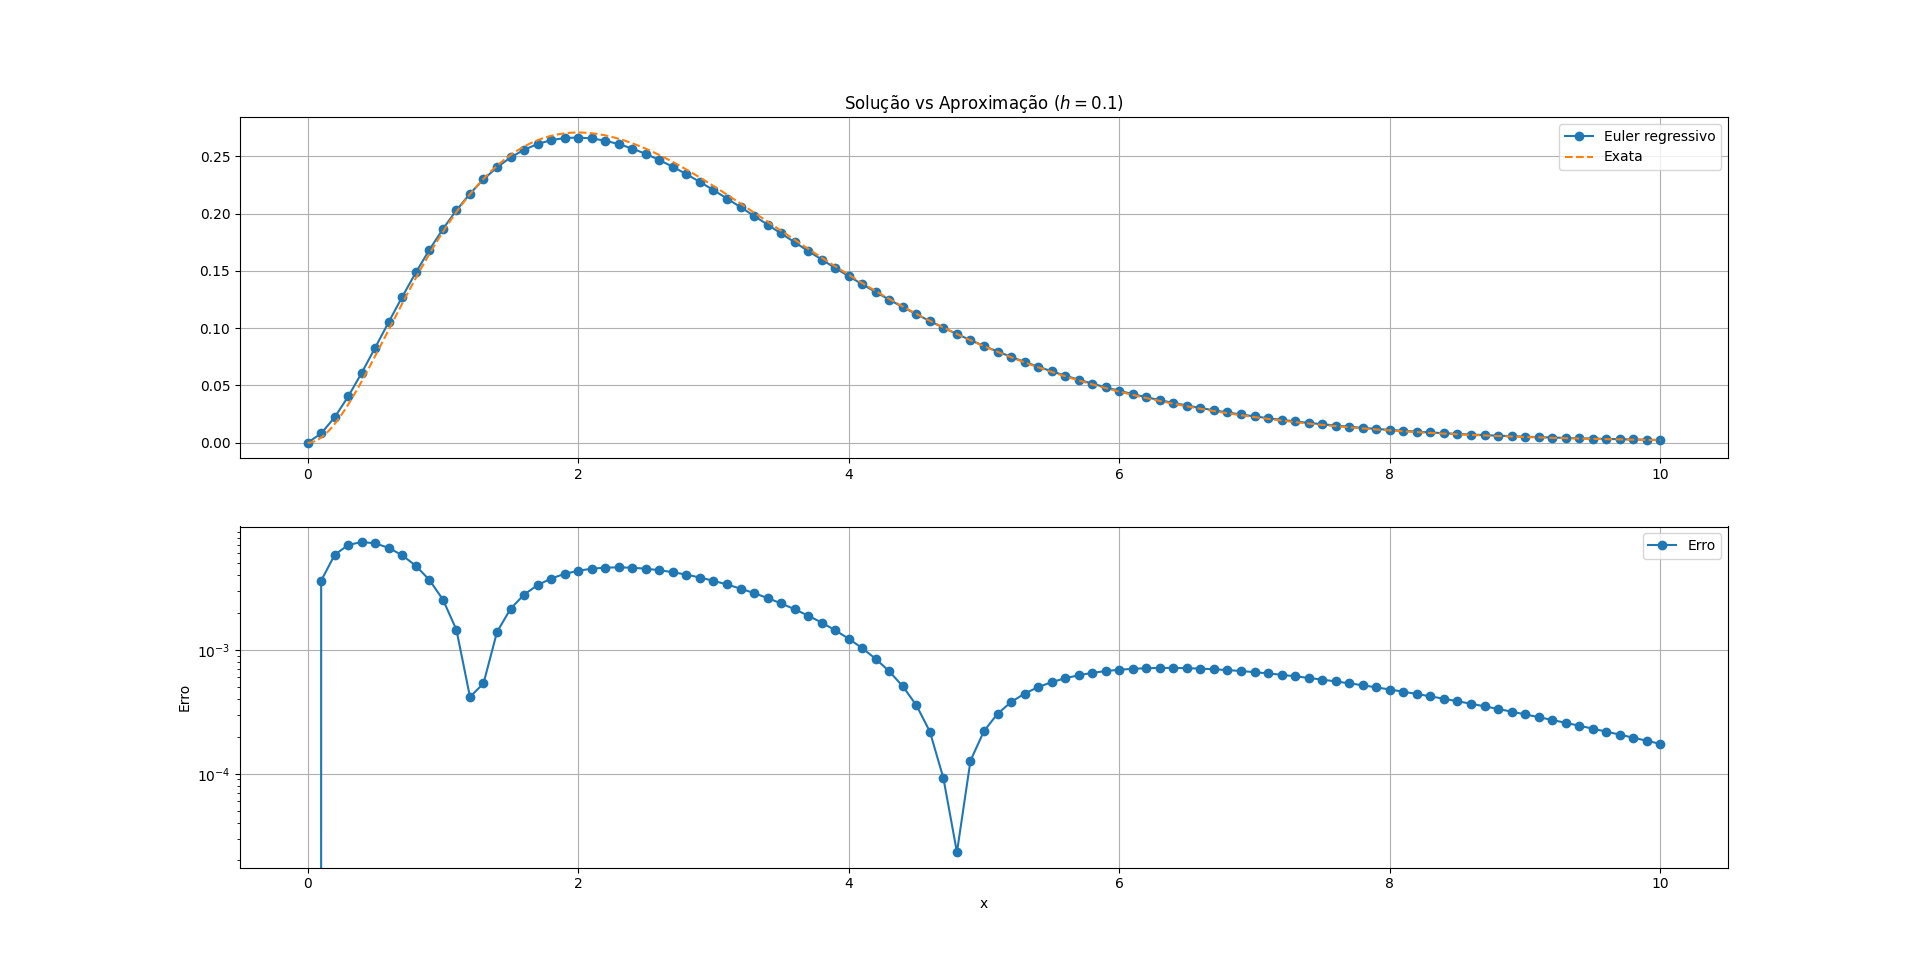
\includegraphics[width=0.7\textwidth]{img/3/implicit_01_2.png}
	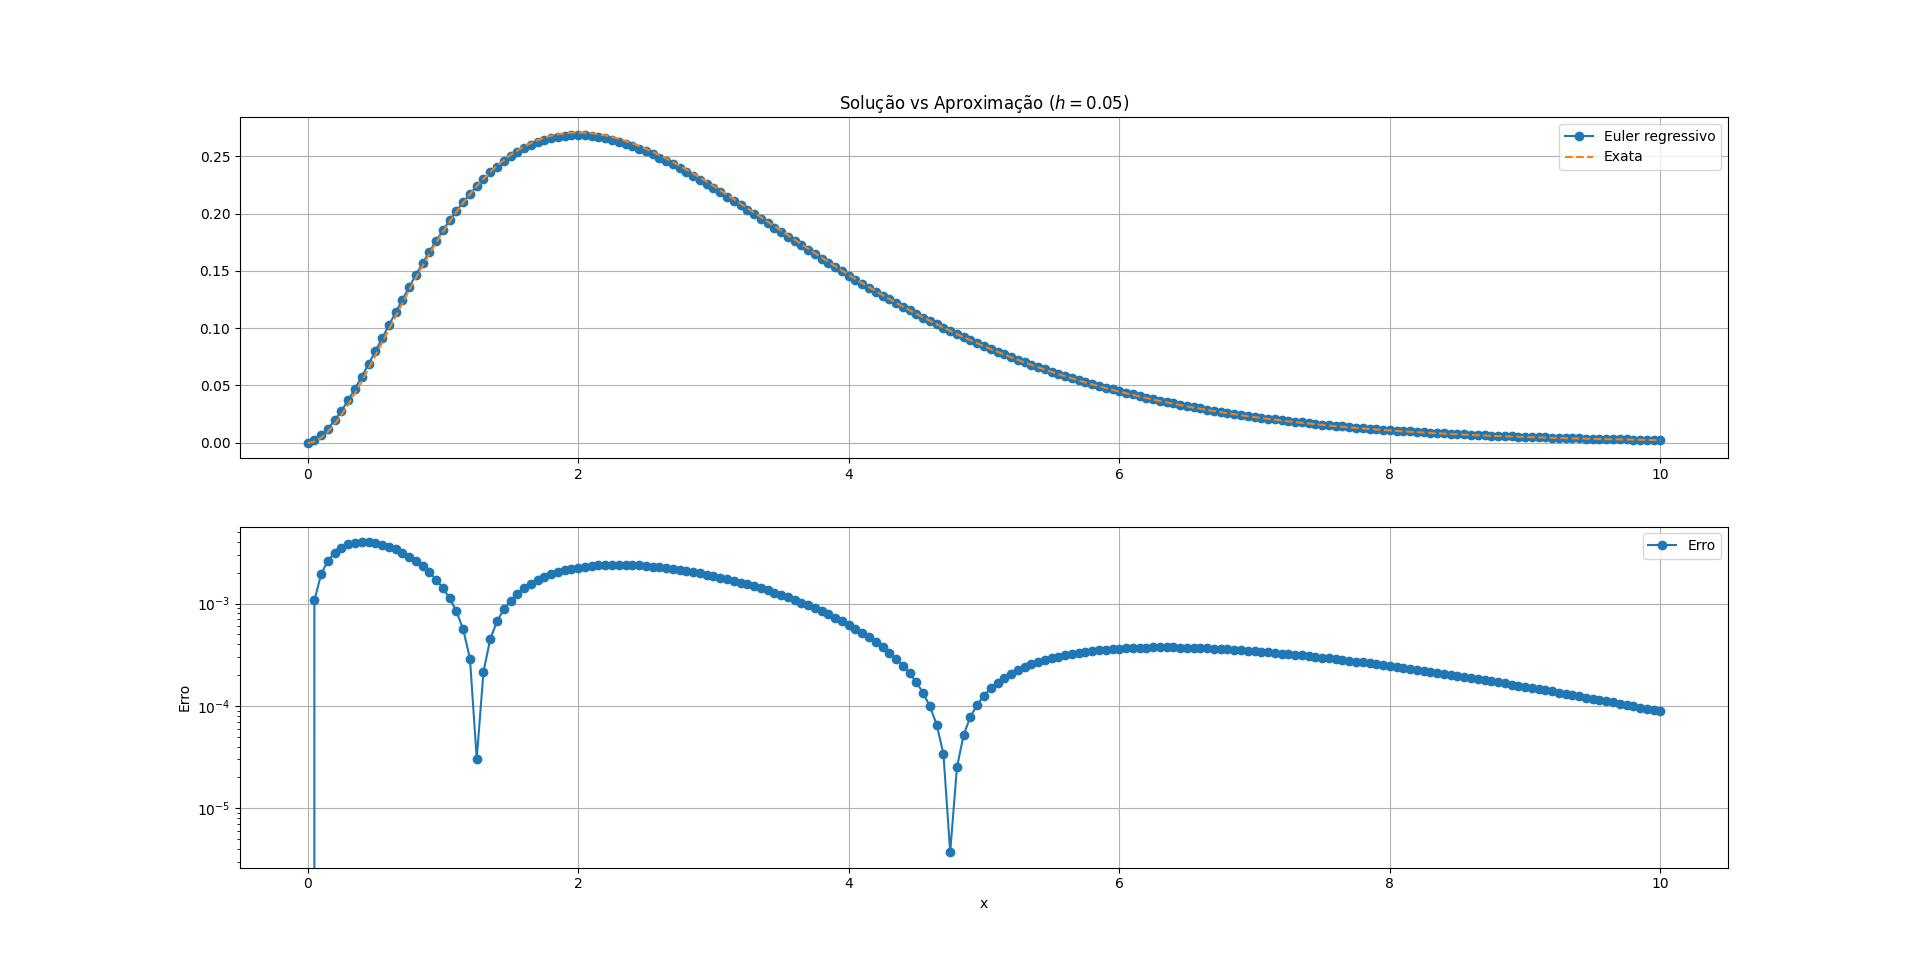
\includegraphics[width=0.7\textwidth]{img/3/implicit_005_2.png}
\end{figure}

\begin{figure}[ht!]
	\centering
	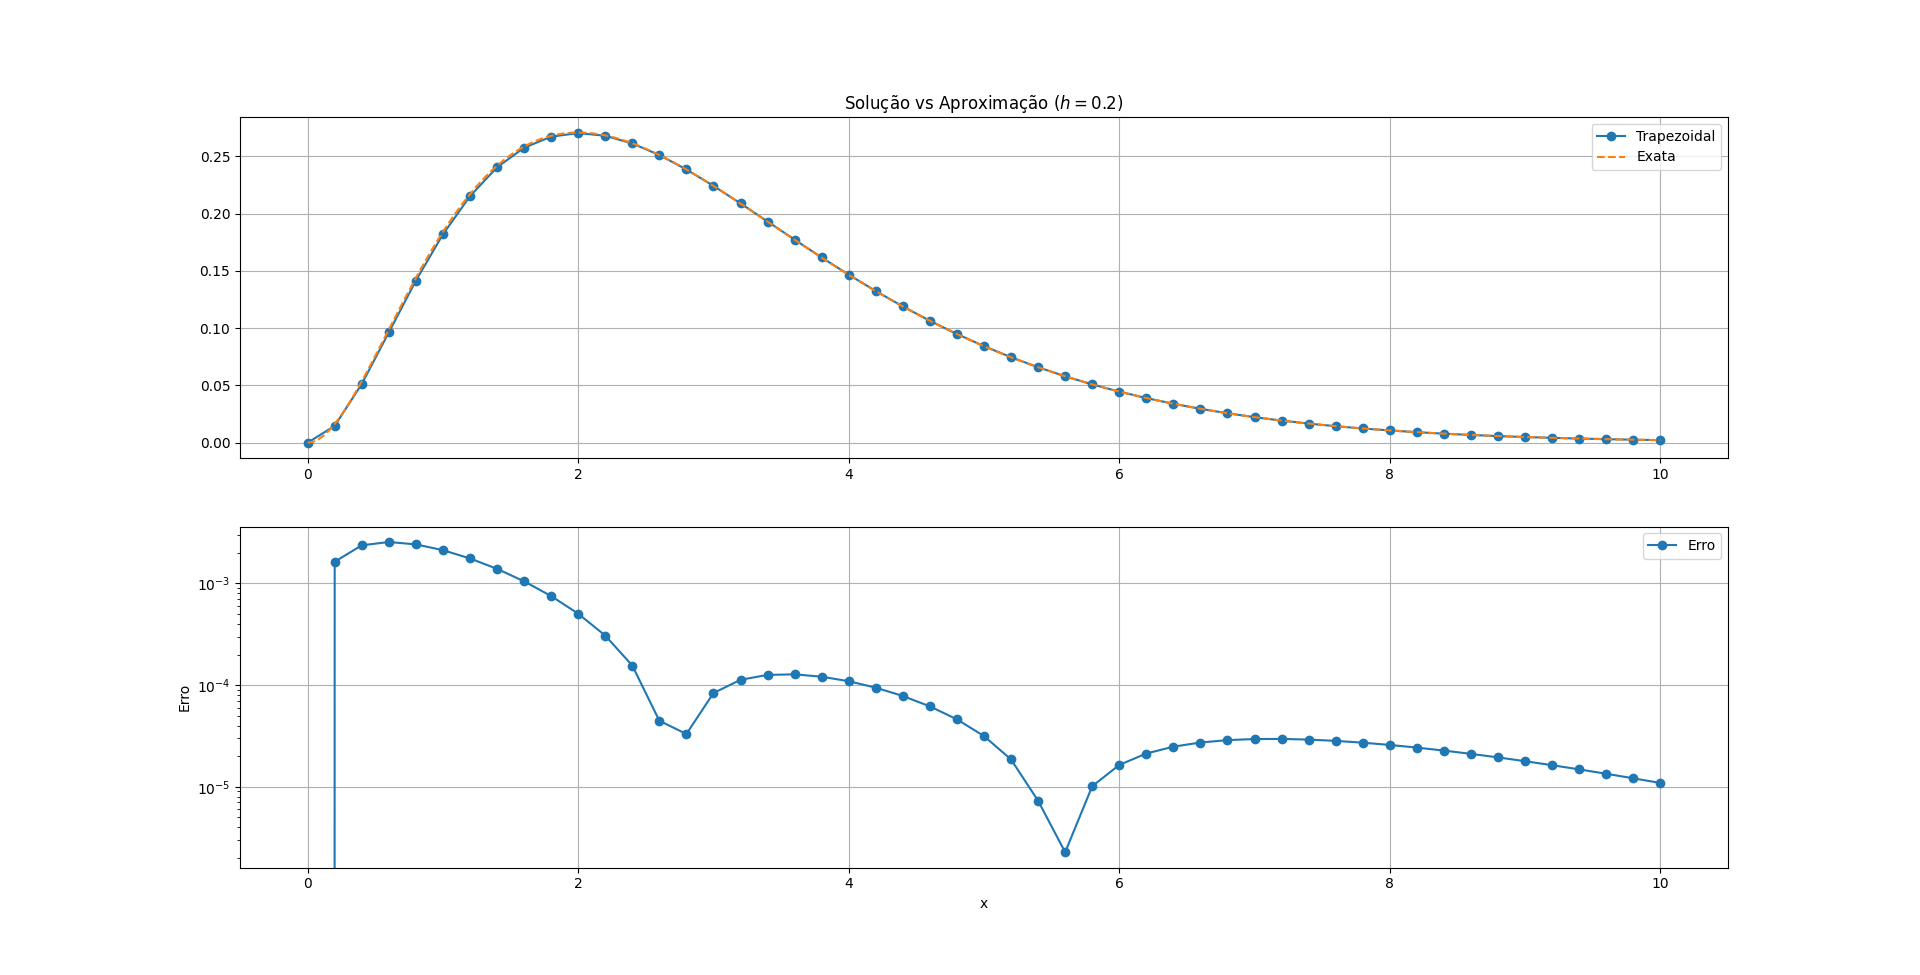
\includegraphics[width=0.7\textwidth]{img/3/trapezoidal_02_2.png}
	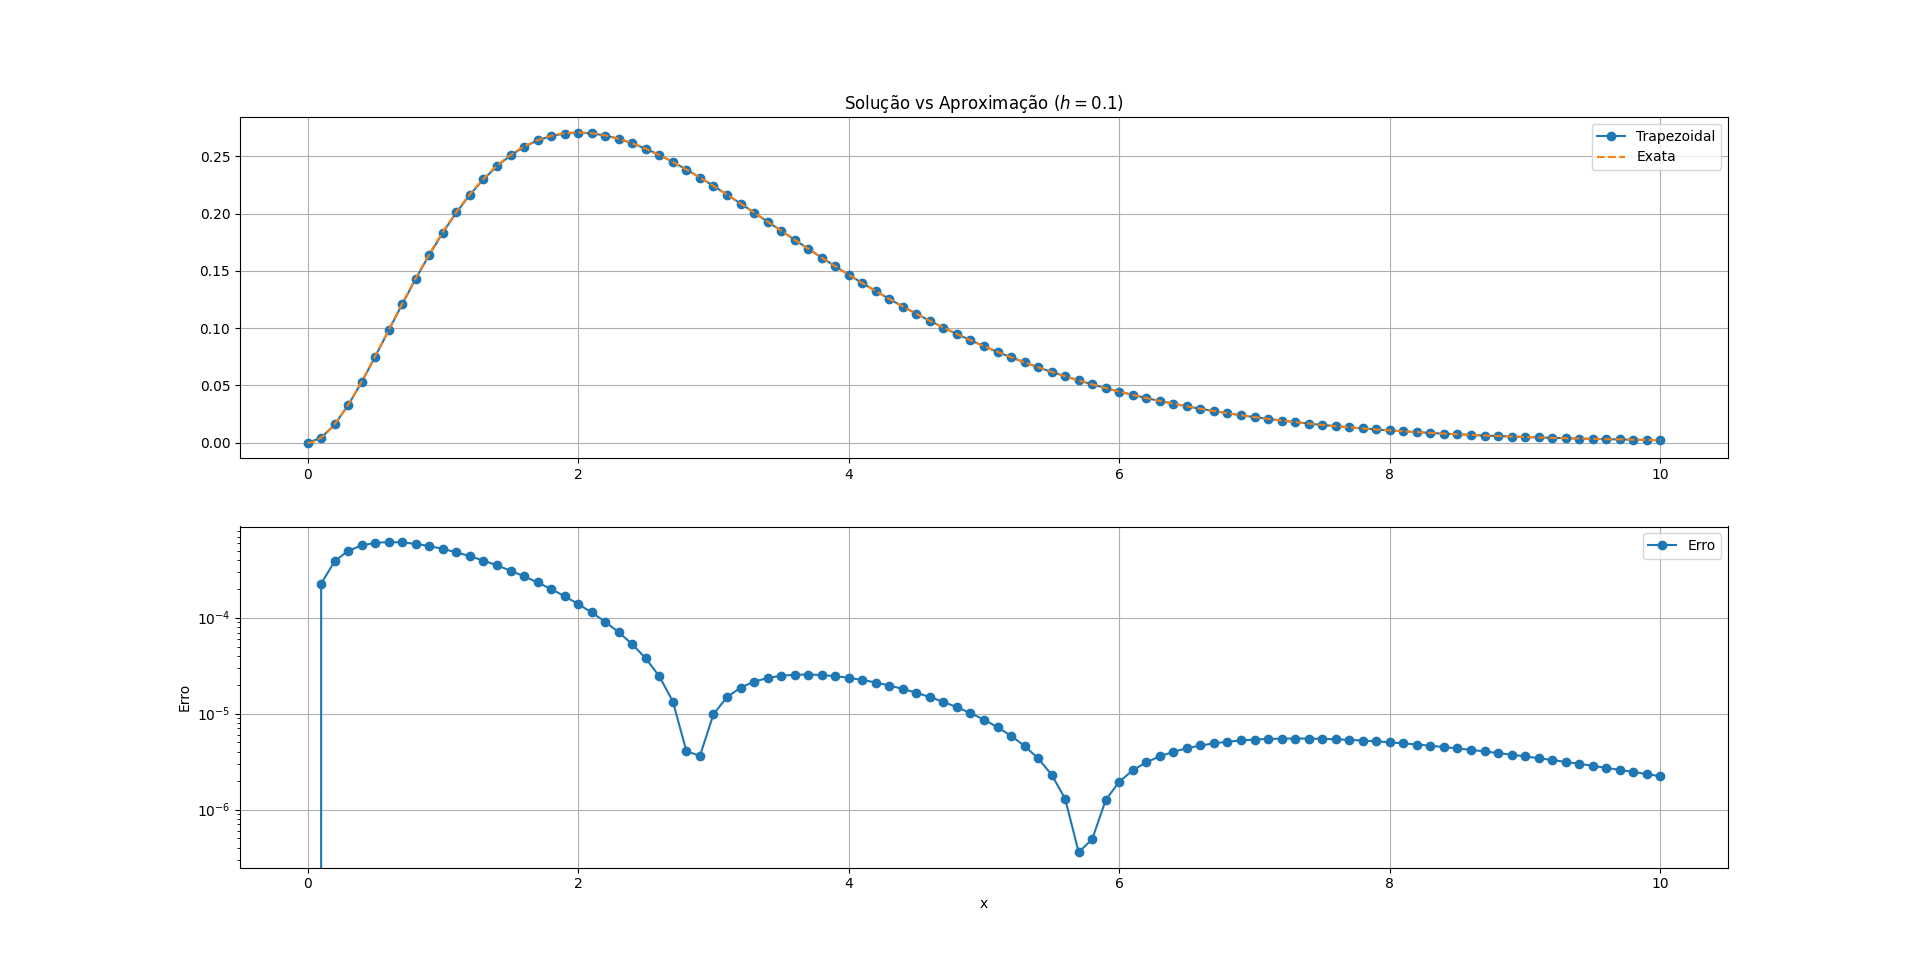
\includegraphics[width=0.7\textwidth]{img/3/trapezoidal_01_2.png}
	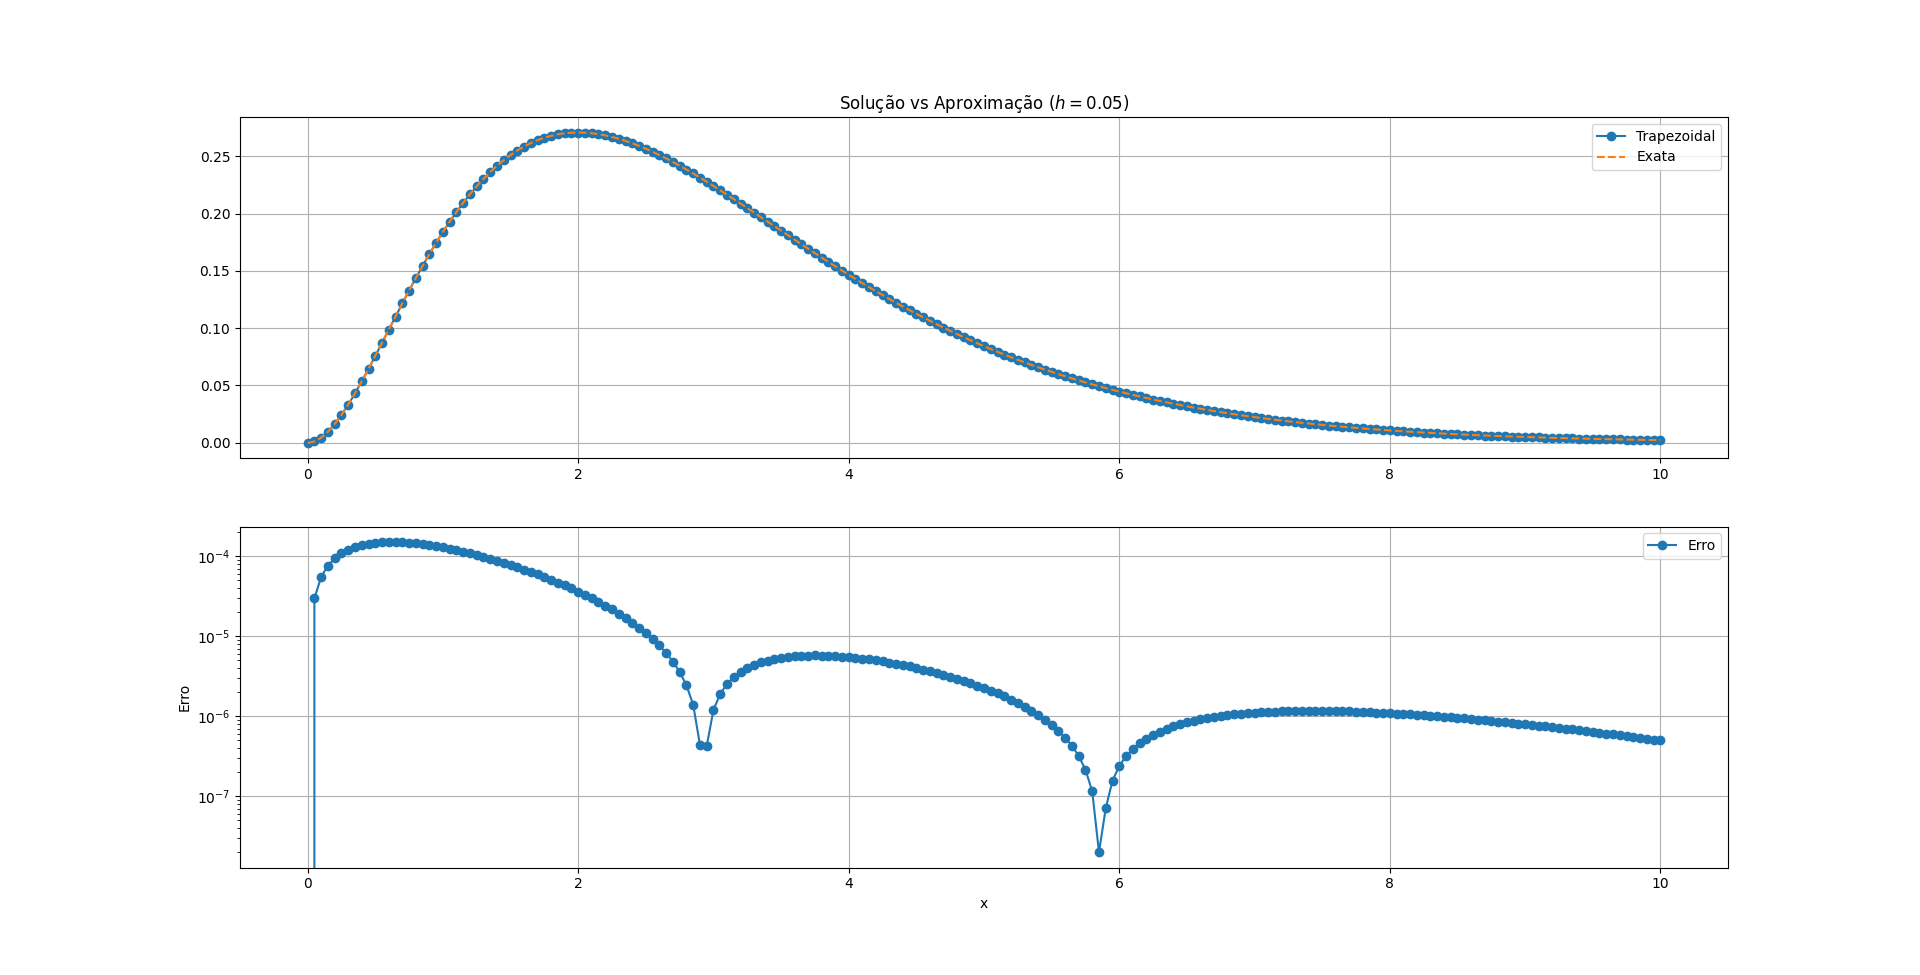
\includegraphics[width=0.7\textwidth]{img/3/trapezoidal_005_2.png}
\end{figure}

\FloatBarrier

\subsection{Implementação de Problemas Não-Lineares}

Tem-se o PVI $y' = -2 y^2; y(1) = 1$, cuja solução exata é $\varphi(x) = \frac{1}{x}$. Todos os métodos discutidos até o momento, tanto implícitos quanto explícitos, podem ser utilizados sem problemas e os erros se comportam de maneira esperada, mesmo a função $f$ sendo não-linear. Seguem os resultados para o método trapezoidal, com 5 correções por iteração (novamente, não houve uma diferença significativa entre 2 e 5 correções).

\begin{figure}[t]
	\centering
	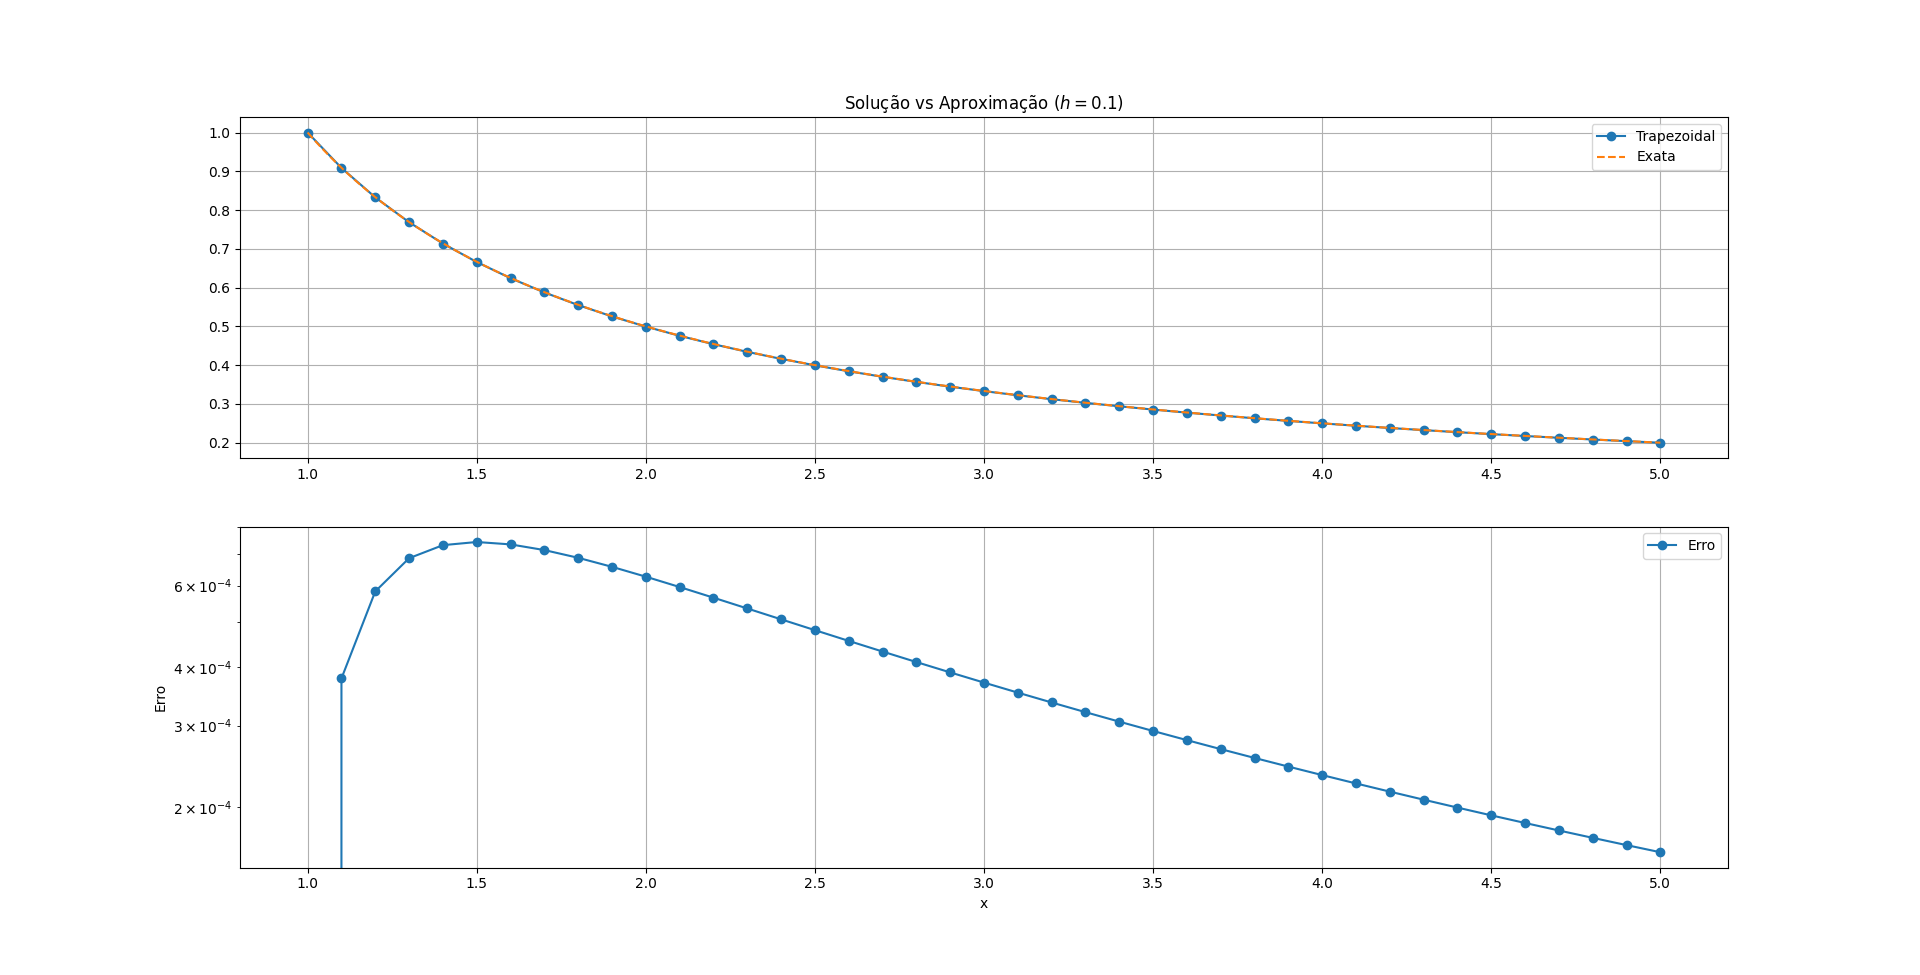
\includegraphics[width=0.9\textwidth]{img/3/nonlinear_trapezoidal_01_5.png}
	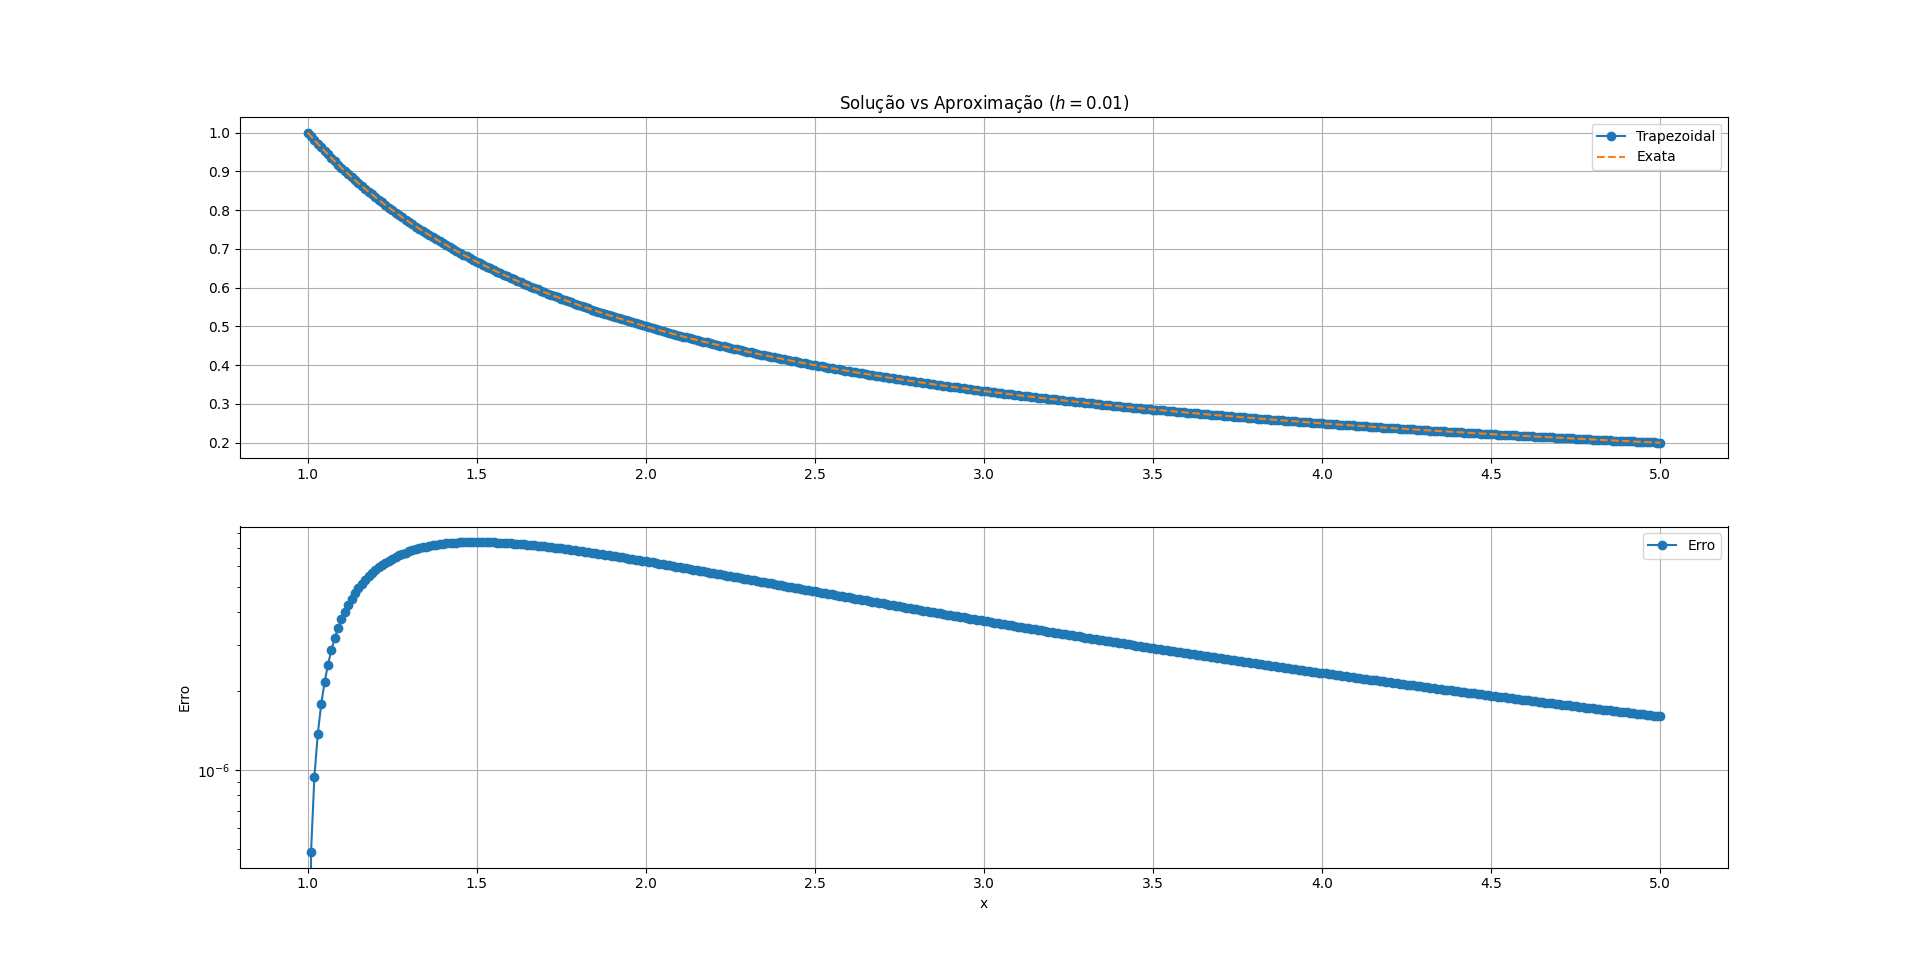
\includegraphics[width=0.9\textwidth]{img/3/nonlinear_trapezoidal_001_5.png}
\end{figure}

Logo, uma das formas possíveis de se implementar é a aplicação direta dos métodos explícitos. No entanto, ao utilizar o método de Euler regressivo, nota-se que cada iteração se torna uma equação quadrática em $y_{j + 1}$. Assim, a fim de evitar as aproximações do esquema preditor-corretor, pode-se resolver a equação direta e achar uma solução exata (em teoria) para o valor de $y_{j + 1}$, em função de $y_j$, sendo então um método explícito.



\end{document}
